%%%%%%%%%%%%%%%%%%%%%%%%%%%%%%%%%%%%%%%%%%%%%%%%%%%%%%%%%%%%%%%%%%%%%%%%%%%%%%%%
% Version Control Systems
%
% Author: Primal Pappachan, FOSSEE 
% Copyright (c) 2012, FOSSEE, IIT Bombay
%%%%%%%%%%%%%%%%%%%%%%%%%%%%%%%%%%%%%%%%%%%%%%%%%%%%%%%%%%%%%%%%%%%%%%%%%%%%%%%%

\documentclass[14pt,compress]{beamer}

\mode<presentation>
{
  \usetheme{Warsaw}
  \useoutertheme{infolines}
  \setbeamercovered{transparent}
}

\usepackage[english]{babel}
\usepackage[latin1]{inputenc}
%\usepackage{times}
\usepackage[T1]{fontenc}

% Taken from Fernando's slides.
\usepackage{ae,aecompl}
\usepackage{mathpazo,courier,euler}
\usepackage[scaled=.95]{helvet}

\definecolor{darkgreen}{rgb}{0,0.5,0}

\usepackage{listings}
\lstset{language=bash,
    basicstyle=\ttfamily\bfseries,
    commentstyle=\color{red}\itshape,
  stringstyle=\color{darkgreen},
  showstringspaces=false,
  keywordstyle=\color{blue}\bfseries}

\newcommand{\inctime}[1]{\addtocounter{time}{#1}{\tiny \thetime\ m}}

\newcommand{\typ}[1]{\lstinline{#1}}

\newcommand{\kwrd}[1]{ \texttt{\textbf{\color{blue}{#1}}}  }

\setbeamercolor{emphbar}{bg=blue!20, fg=black}
\newcommand{\emphbar}[1]

\setbeamertemplate{navigation symbols}{}

\author[Primal Pappachan] {}
\institute[FOSSEE group] {}   

\date[IIT Bombay] {}

\begin{document}

\begin{frame}
\begin{center}
\vspace{12pt}
\textcolor{blue}{\huge Version Control with Mercurial}
\end{center}
\vspace{18pt}
\begin{center}
\vspace{10pt}

\includegraphics[scale=0.95]{../images/fossee-logo.png}\\
\vspace{5pt}
\scriptsize Developed by FOSSEE Team, IIT-Bombay. \\ 
\scriptsize Funded by National Mission on Education through ICT\\
\scriptsize MHRD, Govt. of India.\\

\includegraphics[scale=0.15]{../images/iitb-logo.jpg}\\
\end{center}
\end{frame}

\begin{frame}
  \frametitle{Objectives}
  At the end of this tutorial, you will be able to:
  \begin{itemize}
  \item Understand what is Version Control
  \item Identify the need for using Version Control
  \item Install Mercurial
  \end{itemize}
\end{frame}

%% There are some %$ used just to minimise the effect of $ sign used
%% in lstlisting. In emacs it looks dirty. 

% Introduction to course-need of version control, history, options available.
\section{Introduction}

\begin{frame}
  \frametitle{What is Version Control?}
  \begin{block}{}
    A way to track changes made to files over time, by keeping copies
    of files as we change them.
  \end{block}
\end{frame}

%% Home made version control system?
\begin{frame}[fragile]
  \frametitle{Home-brewed}
  \begin{center}
    An example of a \typ{home-brew} Version Control system
    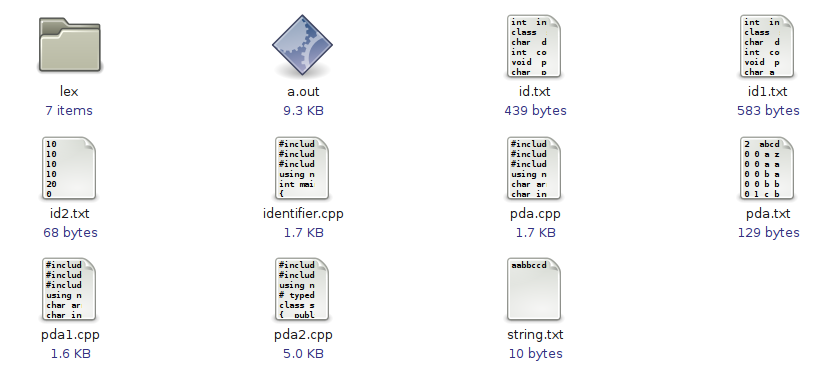
\includegraphics[height=1.8in,width=4.2in]{../images/folder.png}
  \end{center}
  \begin{lstlisting} 
$ ls
a.out  id1.txt  id2.txt  identifier.cpp  id.txt  lex  pda1.cpp  pda2.cpp  pda.cpp  pda.txt  string.txt
  \end{lstlisting} %%$
    %%a screen-shot of folder with all crazy names.
\end{frame}

\begin{frame}[fragile]
  \frametitle{Problems}  
  \begin{block}{}    
  \begin{itemize}
  \item Name and changes made are not related or linked. 
  \item Can't track sequence of changes made to a file. 
  \item Does not scale. 
  \end{itemize}
    \end{block}
\end{frame}

\begin{frame}[fragile]
  \frametitle{The need for Version Control}
  \begin{itemize}
  \item \alert{To err is Human} \ldots 
  \item Tracking the history and evolution of a project
  \item To collaborate effectively on a project
  \item To efficiently track down bugs and pin-point the changes that
    caused it 
  \end{itemize}
\end{frame}

%% Introduction to how logs are managed in VCS.
%% A analogy in logs and day-to-day life?
\begin{frame}[fragile]
  \frametitle{How does it work? --- Analogy}
  It is, in some ways, similar to playing an Video game.
  \begin{itemize}
  \item We play games in stages
  \item Once we finish a stage or a task -- \alert{we SAVE}
  \item We continue playing
  \item But, if necessary, we could choose from one of the saved
    states and start from there
  \item We could alter the course of the game
  \end{itemize}
\end{frame}


\begin{frame}
  \frametitle{Mercurial or \typ{hg}}
  \begin{center}
    
\includegraphics[height=.75in,interpolate=true]{../images/mercurial_logo}
  \end{center}
  \begin{itemize}
  \item Easy to learn and use
  \item Lightweight
  \item Scales excellently
  \item Written in Python
  \end{itemize}
\end{frame}

\begin{frame}
  \frametitle{Installation}
  \begin{itemize}
  \item \typ{sudo apt-get install mercurial}
  \item \typ{\$ hg}
  \item \typ{\$ hg version}
  \end{itemize}
\end{frame}

\begin{frame}[fragile]
\frametitle{Summary...}
In this tutorial, we have learnt about,
\begin{itemize}
\item What is Version Control
\item The need for using Version Control
\item Installing Mercurial or hg
\end{itemize}
\end{frame}

\begin{frame}[fragile]
\frametitle{Evaluation}
\begin{enumerate}
\item Is Mercurial a Centralized VCS or Distributed VCS?
\item How can you verify whether Mercurial has been installed properly?
\item What is the command for accessing built-in help system of Mercurial?
\end{enumerate}
\end{frame}

\begin{frame}
\frametitle{Solutions}
\begin{enumerate}
\item Mercurial is a Distributed Version Control system.
\item hg version  	
\item hg help command	
\end{enumerate}
\end{frame}
\begin{frame}

\begin{block}{}
  \begin{center}
  \textcolor{blue}{\Large THANK YOU!} 
  \end{center}
  \end{block}
\begin{block}{}
  \begin{center}
    For more Information, visit our website\\
    \url{http://fossee.in/}
  \end{center}  
  \end{block}
\end{frame}

\end{document}
